\chapter{Caratteristiche fondamentali del Cloud Computing}
I modelli fondamentali usati per definire servizi, proprietà e fasi del cloud computing si dividono sottocategorie che vanno affrontate separatamente.
\section{Ruoli}
Le organizzazioni e le persone possono assumere diversi tipi di ruoli in base a come si relazionano tra di loro e/o interagiscono con il cloud e le risorse ospitate in rete.
\subsubsection{Cloud Provider}
L'organizzazione che fornisce le risorse IT cloud-based è detta \textbf{Cloud provider}. I cloud provider si occupano di garantire i servizi offerti da un SLA, e di solito posseggono fisicamente le risorse IT che noleggiano; tuttavia ci sono cloud provider che rivendono risorse comprate o noleggiate da altri cloud provider.
\subsubsection{Cloud Consumer}
Un \textbf{cloud consumer} è un'organizzazione o una persona che possiede un contratto formale con un cloud provider per usufruire di certe risorse IT messe a disposizione da quest'ultimo. In particolare, un cloud consumer utilizza un \textit{cloud service consumer} per accedere a un servizio cloud.
\subsubsection{Cloud Service Owner}
È la persona o l'organizzazione che possiede la risorsa IT che mette a dispozione. Può essere anche il cloud consumer stesso, in quanto è colui che istanzia la risorsa.
\subsubsection{Cloud Resource Administrator}
è la persona o l'organizzazione responsabile della gesione delle risorse IT cloud-based. Il Cloud Resource Administrator può essere (o appartenere) il cloud consumer o il cloud provider, oppure può essere un'organizzazione di terze parti entrata in gioco per amministrare le risorse.
\subsubsection{Cloud Auditor}
Una terza parte che conduce valutazioni indipendenti degli ambienti cloud. Le responsabilità del Cloud Auditor includono la valutazione dei controlli di sicurezza e delle garanzie della privacy. Il suo compito principale è quello di fornire una valutazione imparziale dell'ambiente cloud di un cloud provider che verrà utilizzato da un cloud consumer.
\subsubsection{Cloud Broker}
Un Cloud Broker si occupa di negoziare tra le parti; il suo è un ruolo di intermediario tra cloud provider e cloud consumer. I suoi compiti sono principalmente tre:
\begin{itemize}
    \item evitare che un cloud consumer rimanga bloccato da un particolare cloud provider, in modo da poter utilizzare diversi provider per uno stesso servizio;
    \item aggregare i servizi da diversi provider e fornire un servizio uinico che sia una specie di "fusione" tra i vari servizi;
    \item aiutare le aziende a orientarsi tra i vari servizi offerti.
\end{itemize}
\subsubsection{Cloud Carrier}
Il Cloud Carrier è la parte responsabile della fornitura della connessione a livello di rame tra i cloud provider e i cloud consumer. Questo ruolo viene spesso assunto da provider di servizi di rete e di telecomunicazioni.
Il grafico seguente mostra costi e benefici di tutti i ruoli presentati.

\begin{figure}[ht]
    \centering
    
\includegraphics[width=10cm]{./Images/cap3/3.1.png}
    \label{fig:image3.1}
\end{figure}

Il diagramma evidenzia alcune caratteristiche importanti: innanzitutto possiamo distinguere le \textbf{CAPEX} (\textit{capital expenses}, spese in conto capitale), e le \textbf{OPEX} (\textit{operational expenses}, spese operative). 

Possiamo subito notare questo passaggio dai costi iniziali ai benefici, e in particolare possiamo facilmente fare una distizione tra i costi e i prezzi, con i secondi che dipendono direttamente dai primi.
Il creator si occupa dell'infrastruttura, definendo così i costi di fornitura. A questo punto i costi di input influenzano il creator price, che a sua volta influenzano i prezzi successivi fino ad arrivare al business price. Questo infatti viene stabilito dal cloud service consumer che acquista i servizi cloud da rivendere ai clienti. I costi sono rapportati ai benefici, in quanto la costruzione dei prezzi ed il prezzo finale determinano i benefici. I Service Level Agreements garantiscono la QoS che alla fine percepisce l'utente finale.

\section{Boundaries}
Esistono due tipi di boundary:
\begin{itemize}
    \item Un \textbf{Organizational Boundary} è il perimetro fisico che racchiude tutte le risorse IT\footnote{Attenzione: racchiude solo le risorse di natura IT, non rappresenta il limite effettivo dell'organizzazione} possedute e gestite dall'organizzazione.
    \item Un \textbf{Trust Boundary} è un limite esteso per comprendere anche le risorse cloud-based di un'organizzazione.
\end{itemize}
\section{Caratteristiche di un Cloud}
Come già detto, un Cloud non comprende solo risorse IT ma acquista importanza anche in ambito economico. Infatti richiede un insieme specifico di caratteristiche per attivare il remote provisioning e la scalabilità delle risorse in maniera efficiente. La qualità di un Cloud Provider si misura sulle seguenti sei caratteristiche: cinque delle quali prese direttamente dalla definizione di Cloud computing del NIST, a cui viene aggiunta l'ultima per completezza.
\begin{itemize}
    \item on-demand usage (\textit{when});
    \item ubiquitous access (\textit{where});
    \item multitenacy and resource pooling (\textit{how});
    \item elasticity (\textbf{how});
    \item measured usage (\textit{how much});
    \item resiliency (\textit{how reliable}).
\end{itemize}
\subsubsection{On-Demand Usage}
Il Cloud consumer deve poter accedere ai servizi in qualsiasi momento, e effettuare il self-provisioning tramite delle console di gestione dove tutti i servizi possono essere gestiti in maniera autonoma e automatica. Una volta configurata la risorsa non c'è più bisogno di intervento umano.
\subsubsection{Ubiquitous Access}
Rappresenta la possibilità di poter accedere alla risorse tramite più dispositivi o più protocolli di trasporto. In questo modo i servizi sono ritagliati per ogni tipo di consumer, tuttavia man mano che aumenta la user base, aumenta anche il pericolo dei dati che vengono forniti. L'accesso alle risorse è limitato di default, per farantire un accesso più sicuro.
\subsubsection{Multitenancy and Resource Pooling}
È la caratteristica che permette a una risorsa di poter essere utilizzata da più utenti contemporaneamente, ognuno però isolato dall'altro. Essenzialmente si rifà al concetto di virtualizzazione, che permette di isolare processi o anche utenti su un sistema operativo.
In questo modo è possibile dividere la stessa macchina fisica in più macchine virtuali, che quindi vanno a partizionare l'hardware non fisicamente ma logicamente.

\begin{figure}[ht]
    \centering
    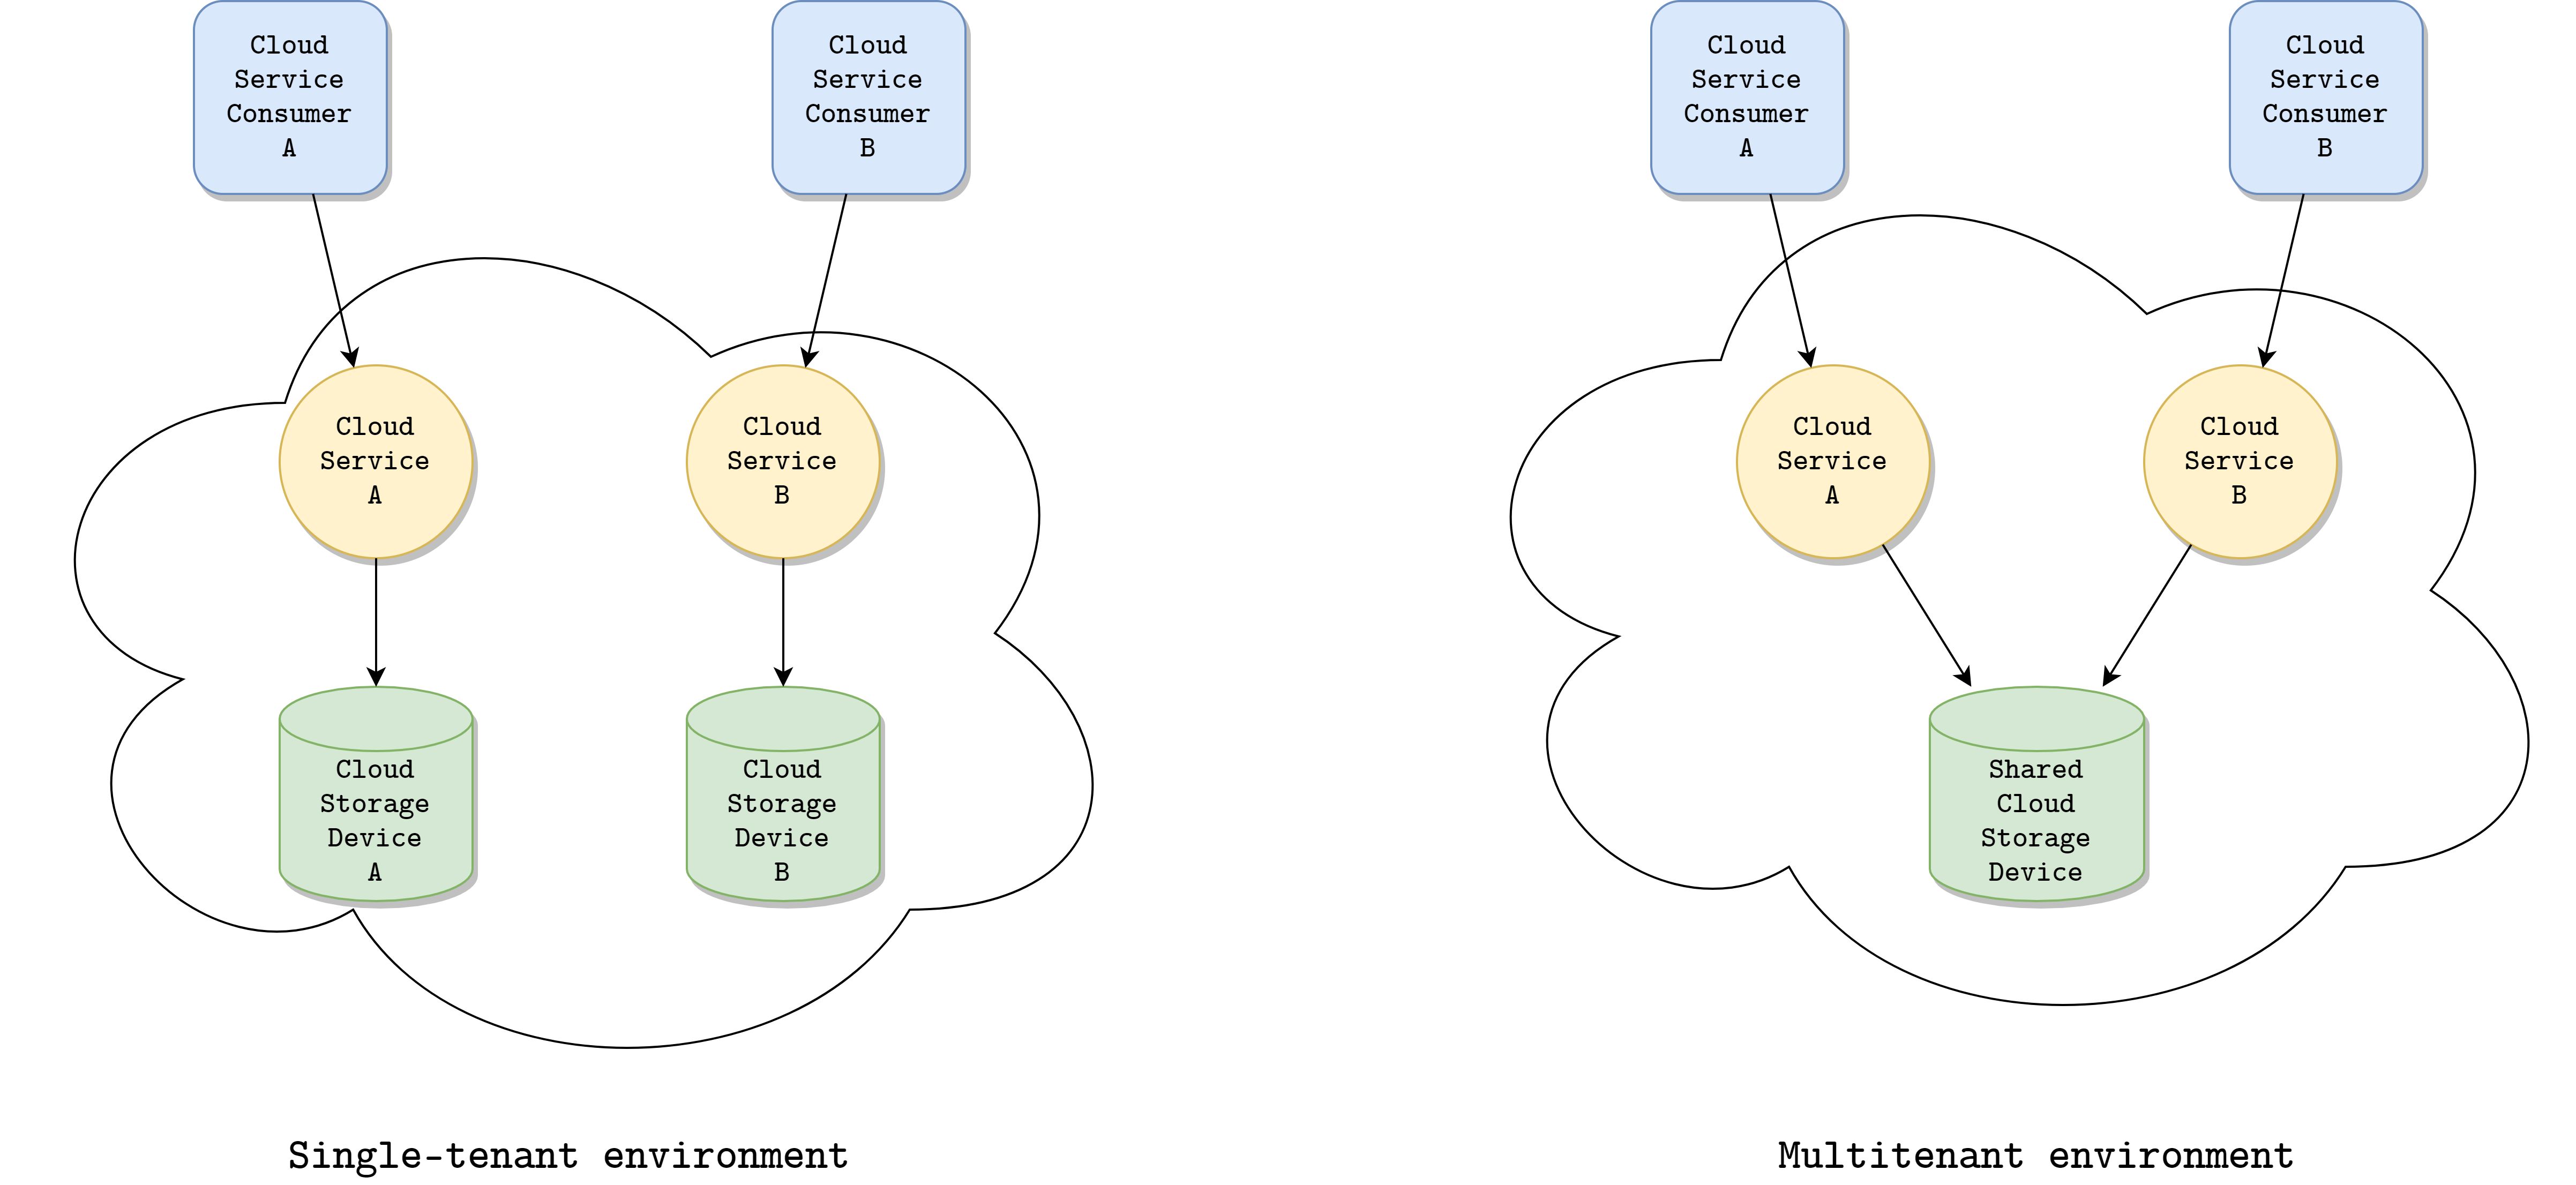
\includegraphics[width=9cm]{./Images/cap3/3.2.png}
    \label{fig:image3.2}
\end{figure}


Il Resource Pooling invece permette ai cloud provider di raggruppare risorse su larga scala in base alla domanda dei consumer. Normalmente questo è possibile sfruttando la multitenancy.

\subsubsection{Rapid Elasticity}
L'elasticity è l'abilità di una piattaforma cloud di scalare in modo trasparente le risorse in base all'aumento o alla diminuzione della domanda. L'elasticity è un aspetto chiave che porta ad adottare le tecniche del cloud computing.

\subsubsection{Measured Usage}
Questa caratteristica permette ad un cloud di tenere traccia dell'utilizzo delle risorse IT. Un consumer in questo modo non paga un servizio con delle quote dipendenti dall'investimento ma solamente dal consumo. Significa che è necessario fornire l'evidenza di qual è l'utilizzo delle risorse, quindi mantenere le informazioni sull'uso ad una grana finissima. Ovviamente è importante non solo per il billing ma anche per il monitoring. Il ruolo che si occupa di questa caratteristica è il Cloud Auditor.
\subsubsection{Resiliency}
Indica quanto è affidabile il servizio ed è la capacità di resistere ai fallimenti. Per fallimenti non si intendono solo quelli di natura informatica ma anche quelli causati da frane, terremoti, disastri naturali che potrebbero compromettere l'integrità di un certo data center. Grazie a questa capacità ci sono meccanismi di failover che permettono di spostare le risorse tra le zone di disponibilità, il tutto mentre il programma è in esecuzione su macchine virtuali. Implica anche la ridondanza di informazioni in diverse su diverse parti del cloud.


\begin{mdframed}[backgroundcolor=gray!20,shadow=false]
\textbf{Summary of Key Points}
\begin{itemize}
    \item L'On-Demand Usage è l'abilità di un cloud consumer di effettuare self-provisioning delle risorse senza l'interazione di un cloud provider.
    \item L'Ubiquitous Access permette ai servizi cloud-based di essere accessi da diversi consumer e da diversi dispositivi, mentre la multitenancy è l'abilità di una singola instanza di risorsa di essere condivisa tra diversi consumer.
\end{itemize}
\end{mdframed}

\section{Cloud Delivery Models}
Un \textit{Cloud Delivery Model} rappresenta una combinazione specifica di risorse IT offerte da un cloud provider. Negli ultimi 10-15 anni si sono distinti principalmente tre modelli:
\begin{itemize}
    \item Infrastructure-as-a-Service (IaaS)
    \item Platform-as-a-Service (PaaS)
    \item Software-as-a-Service (SaaS)
\end{itemize}
Più generalmente, al giorno d'oggi esiste una varietà di questi servizi, che possiamo abbreviare con \textit{x}aaS, dove \textit{x} può rappresentare qualsiasi cosa. In particolare vedremo \textbf{Business Process-as-a-Service} (BPaaS) e \textbf{Information-as-a-Service} (INaaS). 
\subsection{Infrastructure-as-a-Service (IaaS)}
Il modello IaaS presuppone che il cloud consumer sia completamente incaricato della gestione delle risorse: in breve possiede la password della macchina, quindi gestisce i tempi degli aggiornamenti, quando e come deployarli, ecc. \newline
Come si può vedere dal grafico il collegamento tra virtual server e physical server è completamente schermato.

\begin{figure}[ht]
    \centering
    
\includegraphics[width=9cm]{./Images/cap3/3.3.png}
    \label{fig:image3.3}
\end{figure}

\subsection{Platform-as-a-Service (PaaS)}
Il modello Paas permette di avere un pacchetto di risorse pronte all'uso per il cloud consumer. Offre però meno controllo rispetto al modello Iaas. Le risorse offerte per questo tipo di modello sono divise in diversi stack in base all'ambiente e al linguaggio di programmazione usato. 

\begin{figure}[ht]
    \centering
    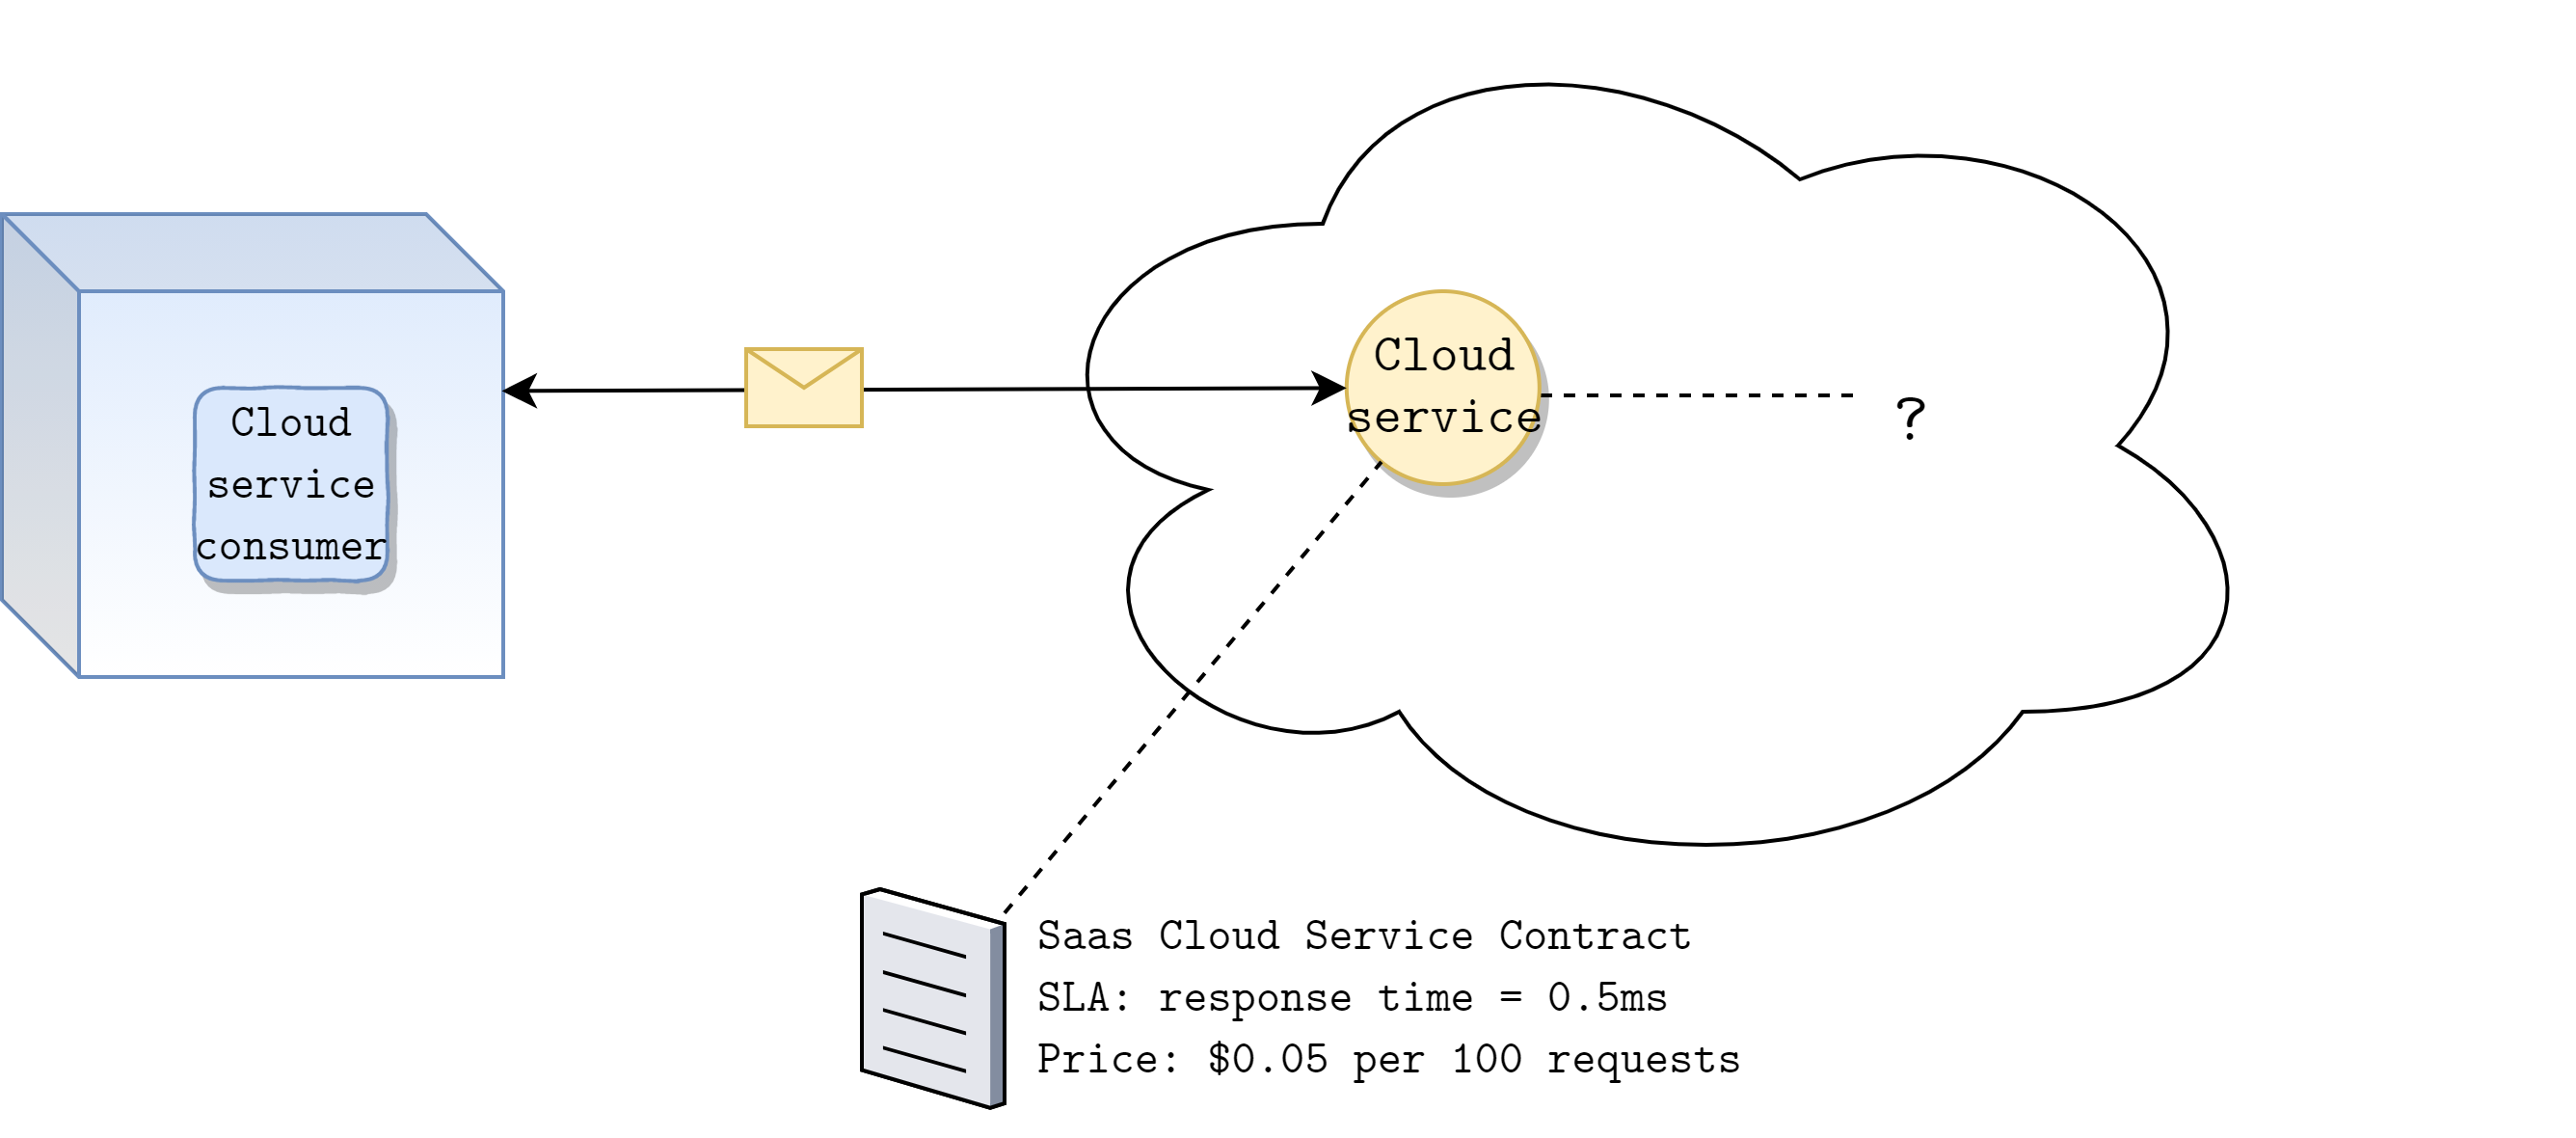
\includegraphics[width=9cm]{./Images/cap3/3.4.png}
    \label{fig:image3.4}
\end{figure}

\subsection{Software-as-a-Service (SaaS)}
Si tratta direttamente di un servizio scritto da altri o dal provider al quale ci si affida. Il cloud consumer non ha nessuna responsabilità per l'amministrazione e non può intervenire. Può essere rappresentato da una RESTful API, da un'applicazione, o da qualsiasi risorsa che mostri solamente l'endpoint attraverso quale si accede.

\subsection{Function-as-a-Service (FaaS)}
È un evoluzione di Iaas e Saas: il cloud consumer non ha l'incombenza di gestire un'infrastruttura, ma ha più libertà di scrivere le applicazioni rispetto a PaaS. Può essere fatto il deployment di funzioni che vengono messe in container forniti dall'infrastruttura del cloud provider. Mentre il vantaggio del consumer è dato dalla libertà di sviluppo, il cloud provider deve bilanciare il carico di lavoro delle risorse rispetto alle richieste e deve farlo alla granularità più fine possibile. 

Ci sono tuttavia delle limitazioni nell'utilizzo della risorsa, ad esempio i tempi di esecuzione o il fatto che si paga ogni volta che la funzione viene invocata. Il modello FaaS può addirittura dare più libertà rispetto a PaaS perché è possibile sviluppare in qualsiasi linguaggio, mentre con PaaS bisogna controllare che il cloud provider offra quel determinato ambiente di sviluppo.

\subsection{Modelli ibridi}
Un modello ibrido come quello IaaS + PaaS  permette di unire i vantaggi di emtrambe le architetture dando molti più vantaggi al cloud consumer. Possono esserci anche due cloud provider diversi a dare le due infrastrutture.

Il modello Iaas + PaaS + SaaS permette invece di combinare diversi livelli di risorse IT costruiti uno sull'altro. In questo modo ogni livello può essere gestito separatamente dagli altri per permettere una gestione più granulata ed efficiente.

\subsection{Business Process-as-a-Service e Information-as-a-Service}
Questi modelli di servizio rappresentano un'estensione del business domain in quanto sono i livelli più astratti dei Delivery Models. Mentre IaaS, PaaS e SaaS sono ormai presenti in ogni Cloud Provider, queste tecnologie vengono inserite in un contesto più orientato al business, che ingloba i modelli precedenti in cui vengono offerti processi di business come servizio. Un esempio è dato dalle aziende che fanno outsourcing delle risorse, ovvero l'esternalizzazione di interi processi aziendali su un'infrastruttura basata su cloud. 

\vspace{5mm}
Tipicamente invece il modello INaaS viene utilizzato da un'azienda che fornisce informazioni legali sui meccanismi di tassazione dell'azienda committente. Questi servizi sono importanti perché rappresentano delivery model se sono su cloud.

\begin{figure}[ht]
    \centering
    
\includegraphics[width=9cm]{./Images/cap3/3.5.png}
    \label{fig:image3.5}
\end{figure}
\newpage
\subsection{Riquadro generale}
Di seguito è possibile osservare un grafico che mostra i diversi livelli di astrazione, e una tabella che mostra le principali differenze tra i diversi modelli.



\begin{table}[ht]
\centering
\begin{tabular}{|l|l|}
\hline
\textbf{Abstraction level}                                                      & \textbf{Service offering}                                                                                                                                                                                                                                                                                                                                                                                               \\ \hline
\begin{tabular}[c]{@{}l@{}}Infrastructure as a \\ service (IaaS)\end{tabular}   & \begin{tabular}[c]{@{}l@{}}Hardware infrastructure (servers, storage, etc.) on a \\ utility basis.\end{tabular}                                                                                                                                                                                                                                                                                                         \\ \hline
\begin{tabular}[c]{@{}l@{}}Platform as a service\\ (PaaS)\end{tabular}          & \begin{tabular}[c]{@{}l@{}}Same as IaaS but includes the operating system\\ and any other core applications of the operating\\ environment to enable you to install and run your\\ software. Pricing generally is on a utility basis.\end{tabular}                                                                                                                                                                      \\ \hline
\begin{tabular}[c]{@{}l@{}}Software as a service\\ (SaaS)\end{tabular}          & \begin{tabular}[c]{@{}l@{}}As per PaaS but includes hosted applications that\\ fulfill a function. The function could be a business,\\ social, or personal function. You simply use the\\ application or applications that you need, when\\ you need it, and avoid the cost of installing and\\ maintaining the application and its supporting\\ hardware infrastructure. Pricing is on a per-use\\ basis.\end{tabular} \\ \hline
\begin{tabular}[c]{@{}l@{}}Information as a \\ service (INaaS)\end{tabular}     & \begin{tabular}[c]{@{}l@{}}Provides information relevant to an individual\\ or corporation and to their businesses, business \\ processes, or tasks. Pricing is usually on a\\ consumption, per-use basis.\end{tabular}                                                                                                                                                                                                 \\ \hline
\begin{tabular}[c]{@{}l@{}}Business process as\\ a service (BPaaS)\end{tabular} & \begin{tabular}[c]{@{}l@{}}Fulfills a business function or replaces a business\\ process in an organization. Typically combines\\ business process outsourcing (BPO) with software\\ as a service (SaaS). Pricing generally on a per use\\ basis.\end{tabular}                                                                                                                                                          \\ \hline
\end{tabular}
\end{table}

\begin{figure}[h!]
    \centering
    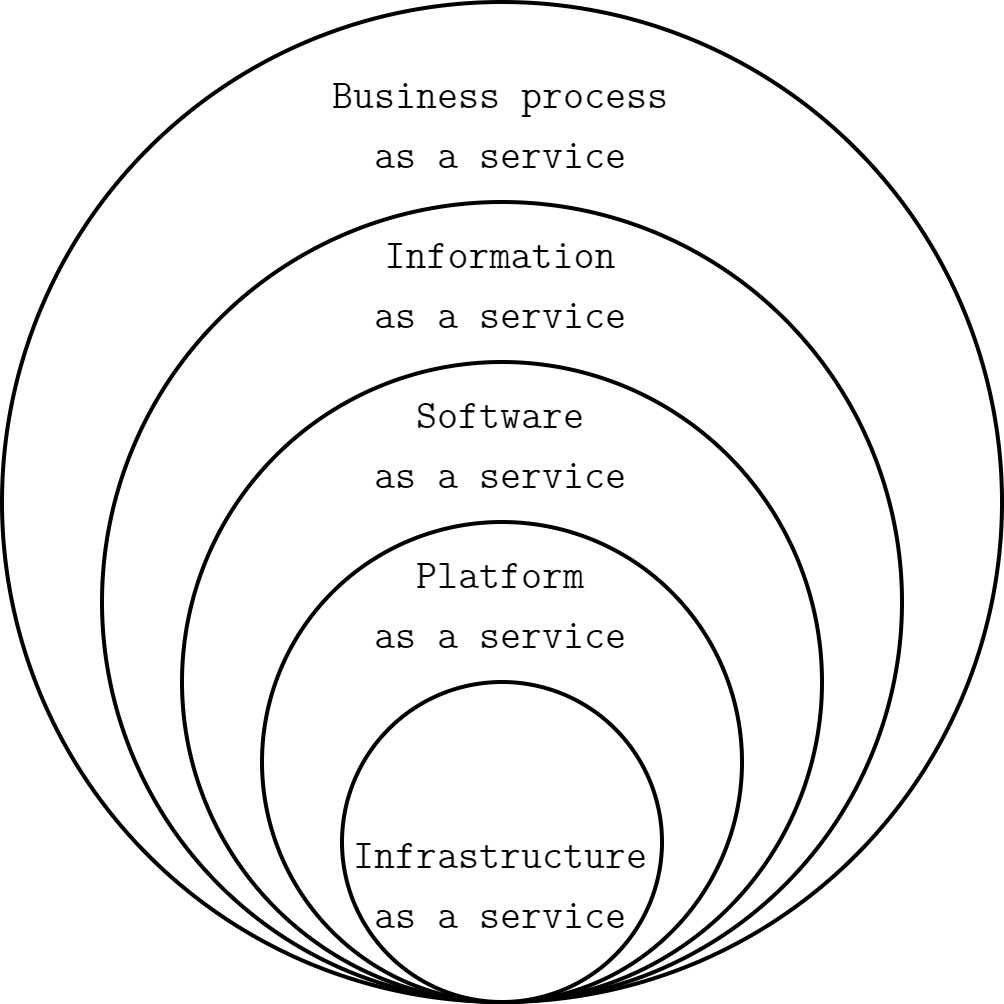
\includegraphics[width=5cm]{./Images/cap3/3.7.png}
\end{figure}

\newpage


\break
\section{Cloud Deployment Models}
I deployment models servono per differenziare gli ambienti per ownership e tipologie di accesso. Distinguiamo 4 modelli:
\begin{itemize}
    \item \textbf{Public Cloud}: è quello più diffuso, consiste nell'utilizzare i servizi messi a disposizione dal cloud provider, che + il responsabile della creazione e la manutenzione delle infrastrutture.
    \item \textbf{Community Cloud}: si tratta di ambienti cloud destinati a una categoria ristretta di utenti: tipicamente utenti che decidono di lavorare insieme sulle stesse caratteristiche di una certa risorsa.
    \item \textbf{Private Cloud}: un cloud privato è gestito da una singola organizzazione per scopi interni, ma che solo poche aziende possono permettersi perché utilizza un gran numero di risorse e attrezzature. Organizzativamente è omogeneo, quindi il cloud diventa una risorsa formalmente esportata verso un altro dipartimento. Attenzione perché questo non vuol dire che le risorse sono on-premise, perché anche il private cloud offre le caratteristiche di resilienza ed elasticità che spesso le risorse on-premise non hanno. La cosa fondamentale è capire come funziona: spesso sono le aziende che acquistano infrastrutture da un cloud provider e le mettono a disposizione della propria azienda, da come si può vedere nel grafico.
    
    \begin{figure}[ht]
    \centering
    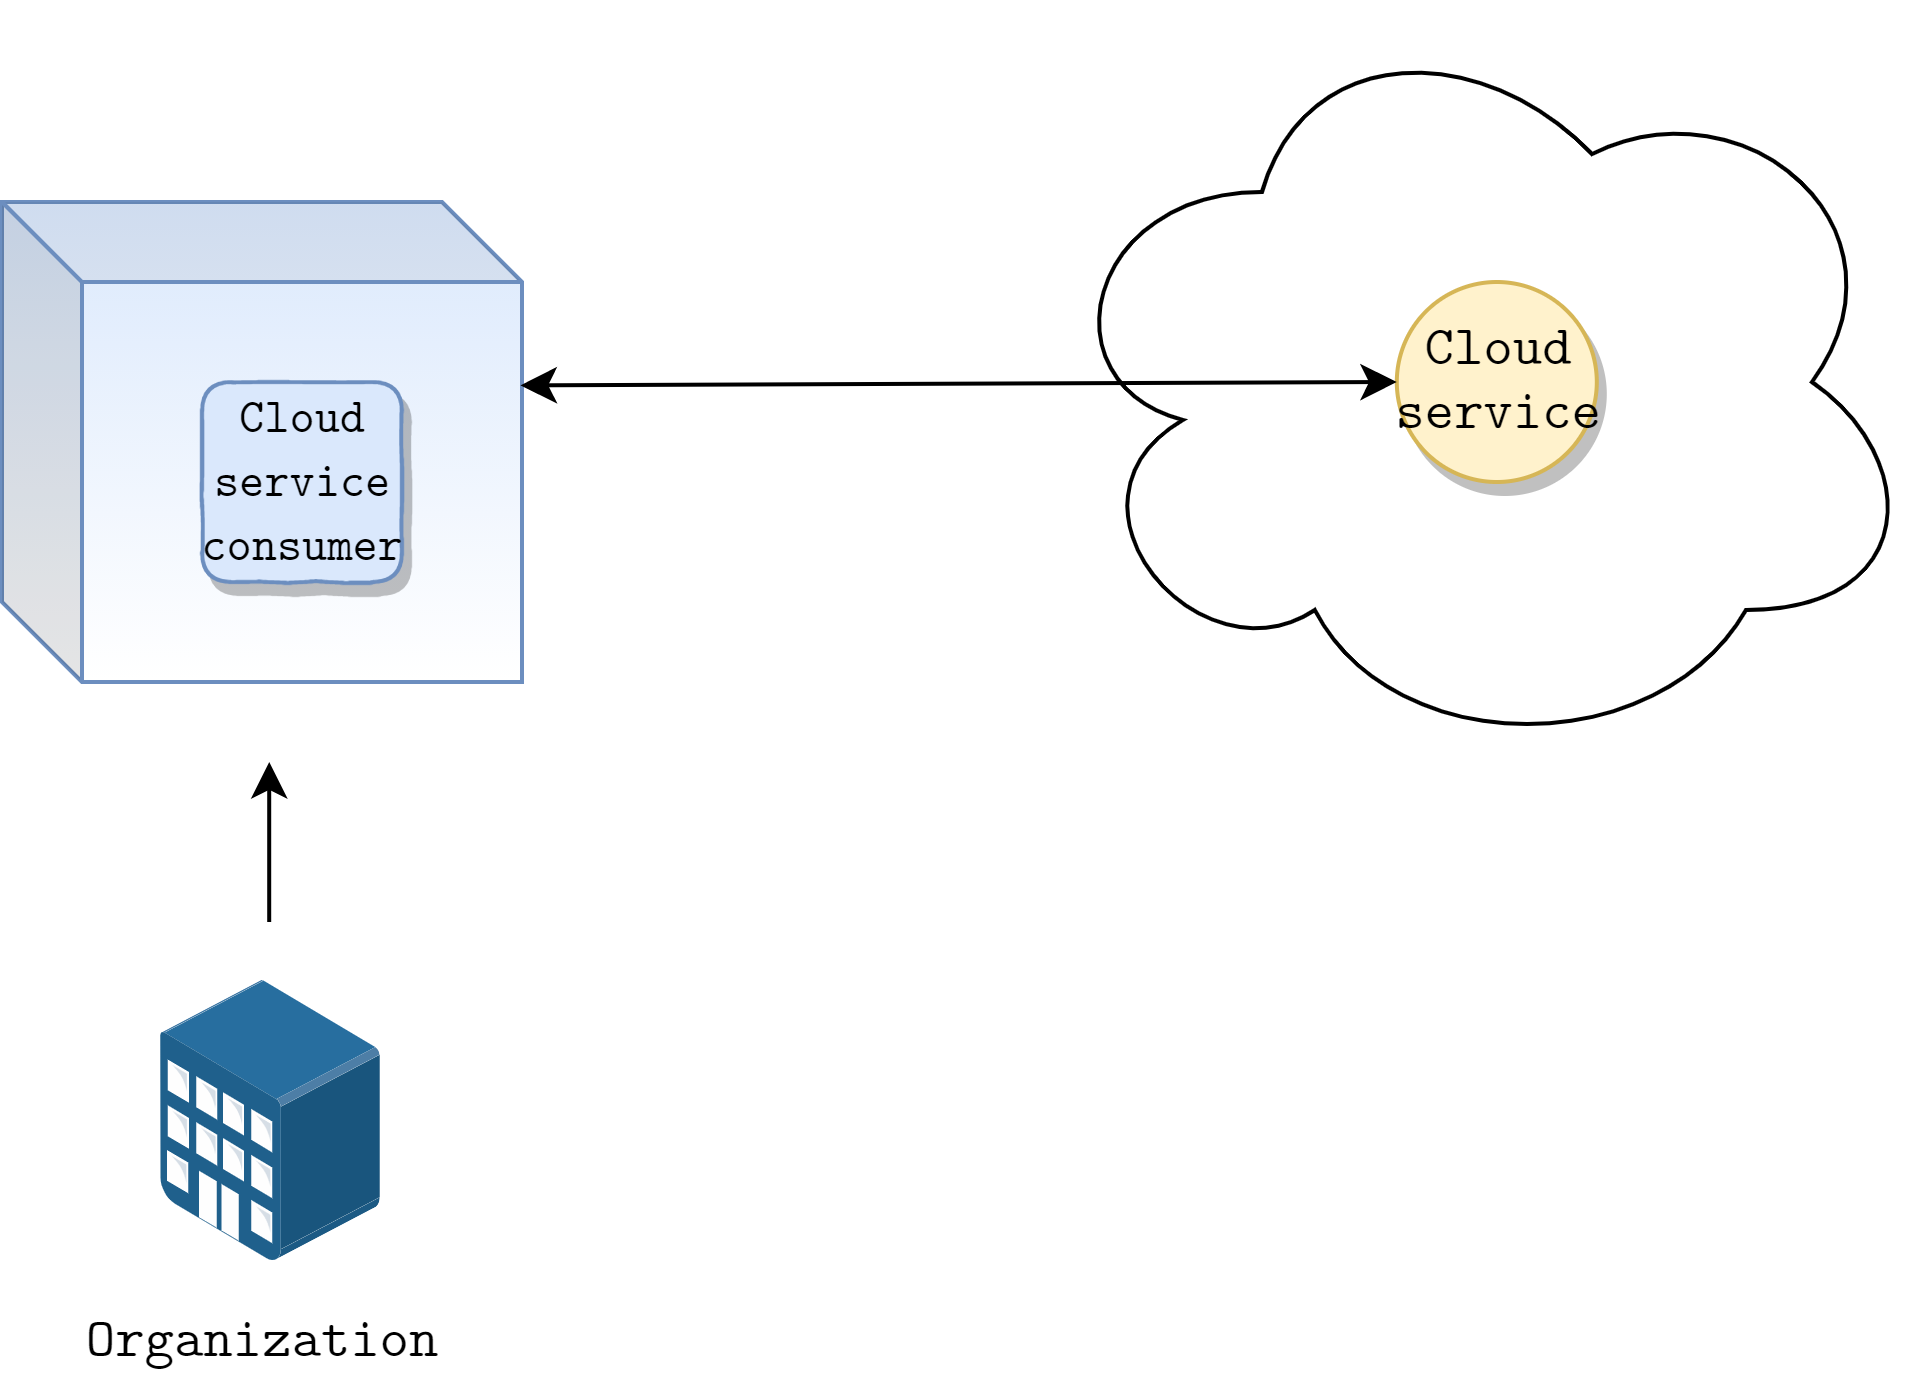
\includegraphics[width=8cm]{./Images/cap3/3.6.png}
    \label{fig:image3.6}
    \end{figure}
    
    Infatti una risorsa on-premise non è un servizio. Un cloud privato è vantaggioso perché risiede all'interno di del trust boundary di un'azienda. È comodo per avere più controllo sui dati, ed ha il vantaggio di estrarre i processi che normalmente non si può fare con le risorse on-premise, soprattutto quelli di billing e di measured usage per sapere i costi precisi.
    
    \item \textbf{Hybrid Cloud}: un cloud ibrido permette ad un'organizzazione di utizzare sia un cloud privato che quello pubblico in modo da scalare più facilmente, avendo a disposizione risorse maggiori di quelle presenti all'interno dell'azienda. 
\end{itemize}

\section{Learning Check}
\begin{enumerate}
    \item Descrivi i ruoli che si applicano agli individui, alle organizzazioni e ai software che fanno parte di un ambiente cloud, includendo: service consumer, cloud service consumer, cloud provider, cloud consumer, cloud service owner, cloud resource administrator.
    \item Descrivi i limiti fisici e logici di un ambiente cloud, includendo gli Organizational boundary (in relazione ai cloud provider e ai cloud consumer), e i Trust boundary (e come sono in relazione tra cloud consumer e cloud provider). Spiega anche la relazione tra questi due tipi di boundaries.
    \item Elenca e descrivi l'insieme delle caratteristiche che deve avere un ambiente IT per essere considerato un cloud.
    \item Descrivi le caratteristiche dell On-Demand Usage e come si relaziona allo scaling.
    \item Descrivi le caratteristiche dell'Ubiquitous Access.
    \item Descrivi la caratteristica del multitenancy in relazione all'allocazione di risorse IT.
    \item Descrivi le caratteristiche dell'Elasticity e come è associata all'aumento degli investimenti e ai costi proporzionali.
    \item Descrivi le caratteristiche del Measured Usage e come si relaziona col modello pay-per-use.
    \item Descrivi le caratteristiche della Resiliency e come si relaziona ai failover.
    \item Descrivi il modello Iaas e come si collega al provisioning delle risorse "raw". Spiega anche come i cloud consumer guadagnano un alto livello di controllo con il modello IaaS.
    \item Descrivi il modello PaaS e come fornisce un ambiente cloud predefinito.
    \item Descrivi il modello SaaS e come limita il controllo del cloud consumer.
    \item Spiega come possono essere mescolati i modelli di cloud delivery.
    \item Descrivi il modello di deployment di cloud pubblico e spiega come le risorse IT di un cloud pubblico sono fornite da una terza parte a pagamento.
    \item Descrivi il modello di community cloud e spiega come l'accesso è limitato a un insieme ristretto di utenti.
    \item Descrivi il modello di cloud privato e spiega come un cloud privato è posseduto da una singola organizzazione.
    \item Descrivi il modello di cloud ibrido e spiega perché un cloud è detto \textit{ibrido} in relazione agli altri modelli.
\end{enumerate}


\begin{comment}
IL CAPITOLO CHE FINISCE QUA IN REALTA ERA ANCORA IL 2, ORA INIZIA IL 3
\end{comment}

\chapter{Tecnologie chiave del Cloud Computing}
Come già detto in precedenza, è importante comprendere gli aspetti del fenomeno del cloud computing non solo come un fenomeno tecnologico, ma anche e principalmente economico. Infatti il cloud come lo conosciamo oggi ha avuto delle spinte economiche di grande portata. Ad esempio, come appena visto, un cloud privato gestisce le spese meglio rispetto ad una infrastruttura on premise, questo perché viene fatto accounting e billing stesso all'interno dell'azienda, rendendo tutti consapevoli dei costi e degli investimenti. In pratica il cloud privato tratta i dipendenti dell'azienda come se fossero clienti.

\vspace{5mm}

Le tecnologie che vedremo in questo capitolo vengono considerate importanti per aver costituito il cloud, ma solo se prese tutte insieme, in quanto singolarmente non influiscono in maniera decisiva. Alcune di queste tecnologie esistevano già prima del cloud, ma messe insieme sono diventate mature nello stesso momento, e hanno reso possibile quel movimento che ha portato alla fornitura di capacità di calcolo come servizio. Distinguiamo sei tecnologie chiave:
\begin{itemize}
    \item \textbf{Broadband Networks and Internet Architecture}
    \item \textbf{Data Center Technology}
    \item \textbf{Virtualization Technology}
    \item \textbf{Web Technology}
    \item \textbf{Multitenant Technology}
    \item \textbf{Service Technology}
\end{itemize}
\section{Broadband Networks and Internet Architecture}
Uno dei principi fondamentali del cloud computing è la possibilità di accedervi ovunque, e ciò implica connettività di rete, requisito quindi critico per il corretto funzionamento. Anche nel caso di cloud che permettono di gestire una parte delle risorse offline, la rete è comunque necessaria per effettuare il \textit{remote provisioning} delle risorse.

\subsection{Funzionamento della rete}
Gli ISP hanno il compito di fare da backbone a tutte le reti, collegandole tra di loro. Come illustra il grafico, partendo dall'altro si può notare come il cloud consumer, che in questo caso è un'organizzazione, ha una rete da cui accede ben strutturata. Le comunicazioni con l'esterno avvengono tramite gli ISP che con la loro struttura modulare si occupano di gestire un'enorme quantità di traffico di rete. Il backbone connette anche i service provider a cui il cloud provider è collegato. Qui si vede anche la centralità del ruolo del \textbf{Cloud Carrier}, che offre ridondanza a livello di gestione per garantire la qualità della rete anche in caso di malfunzionamenti. 

\begin{figure}[ht]
    \centering
    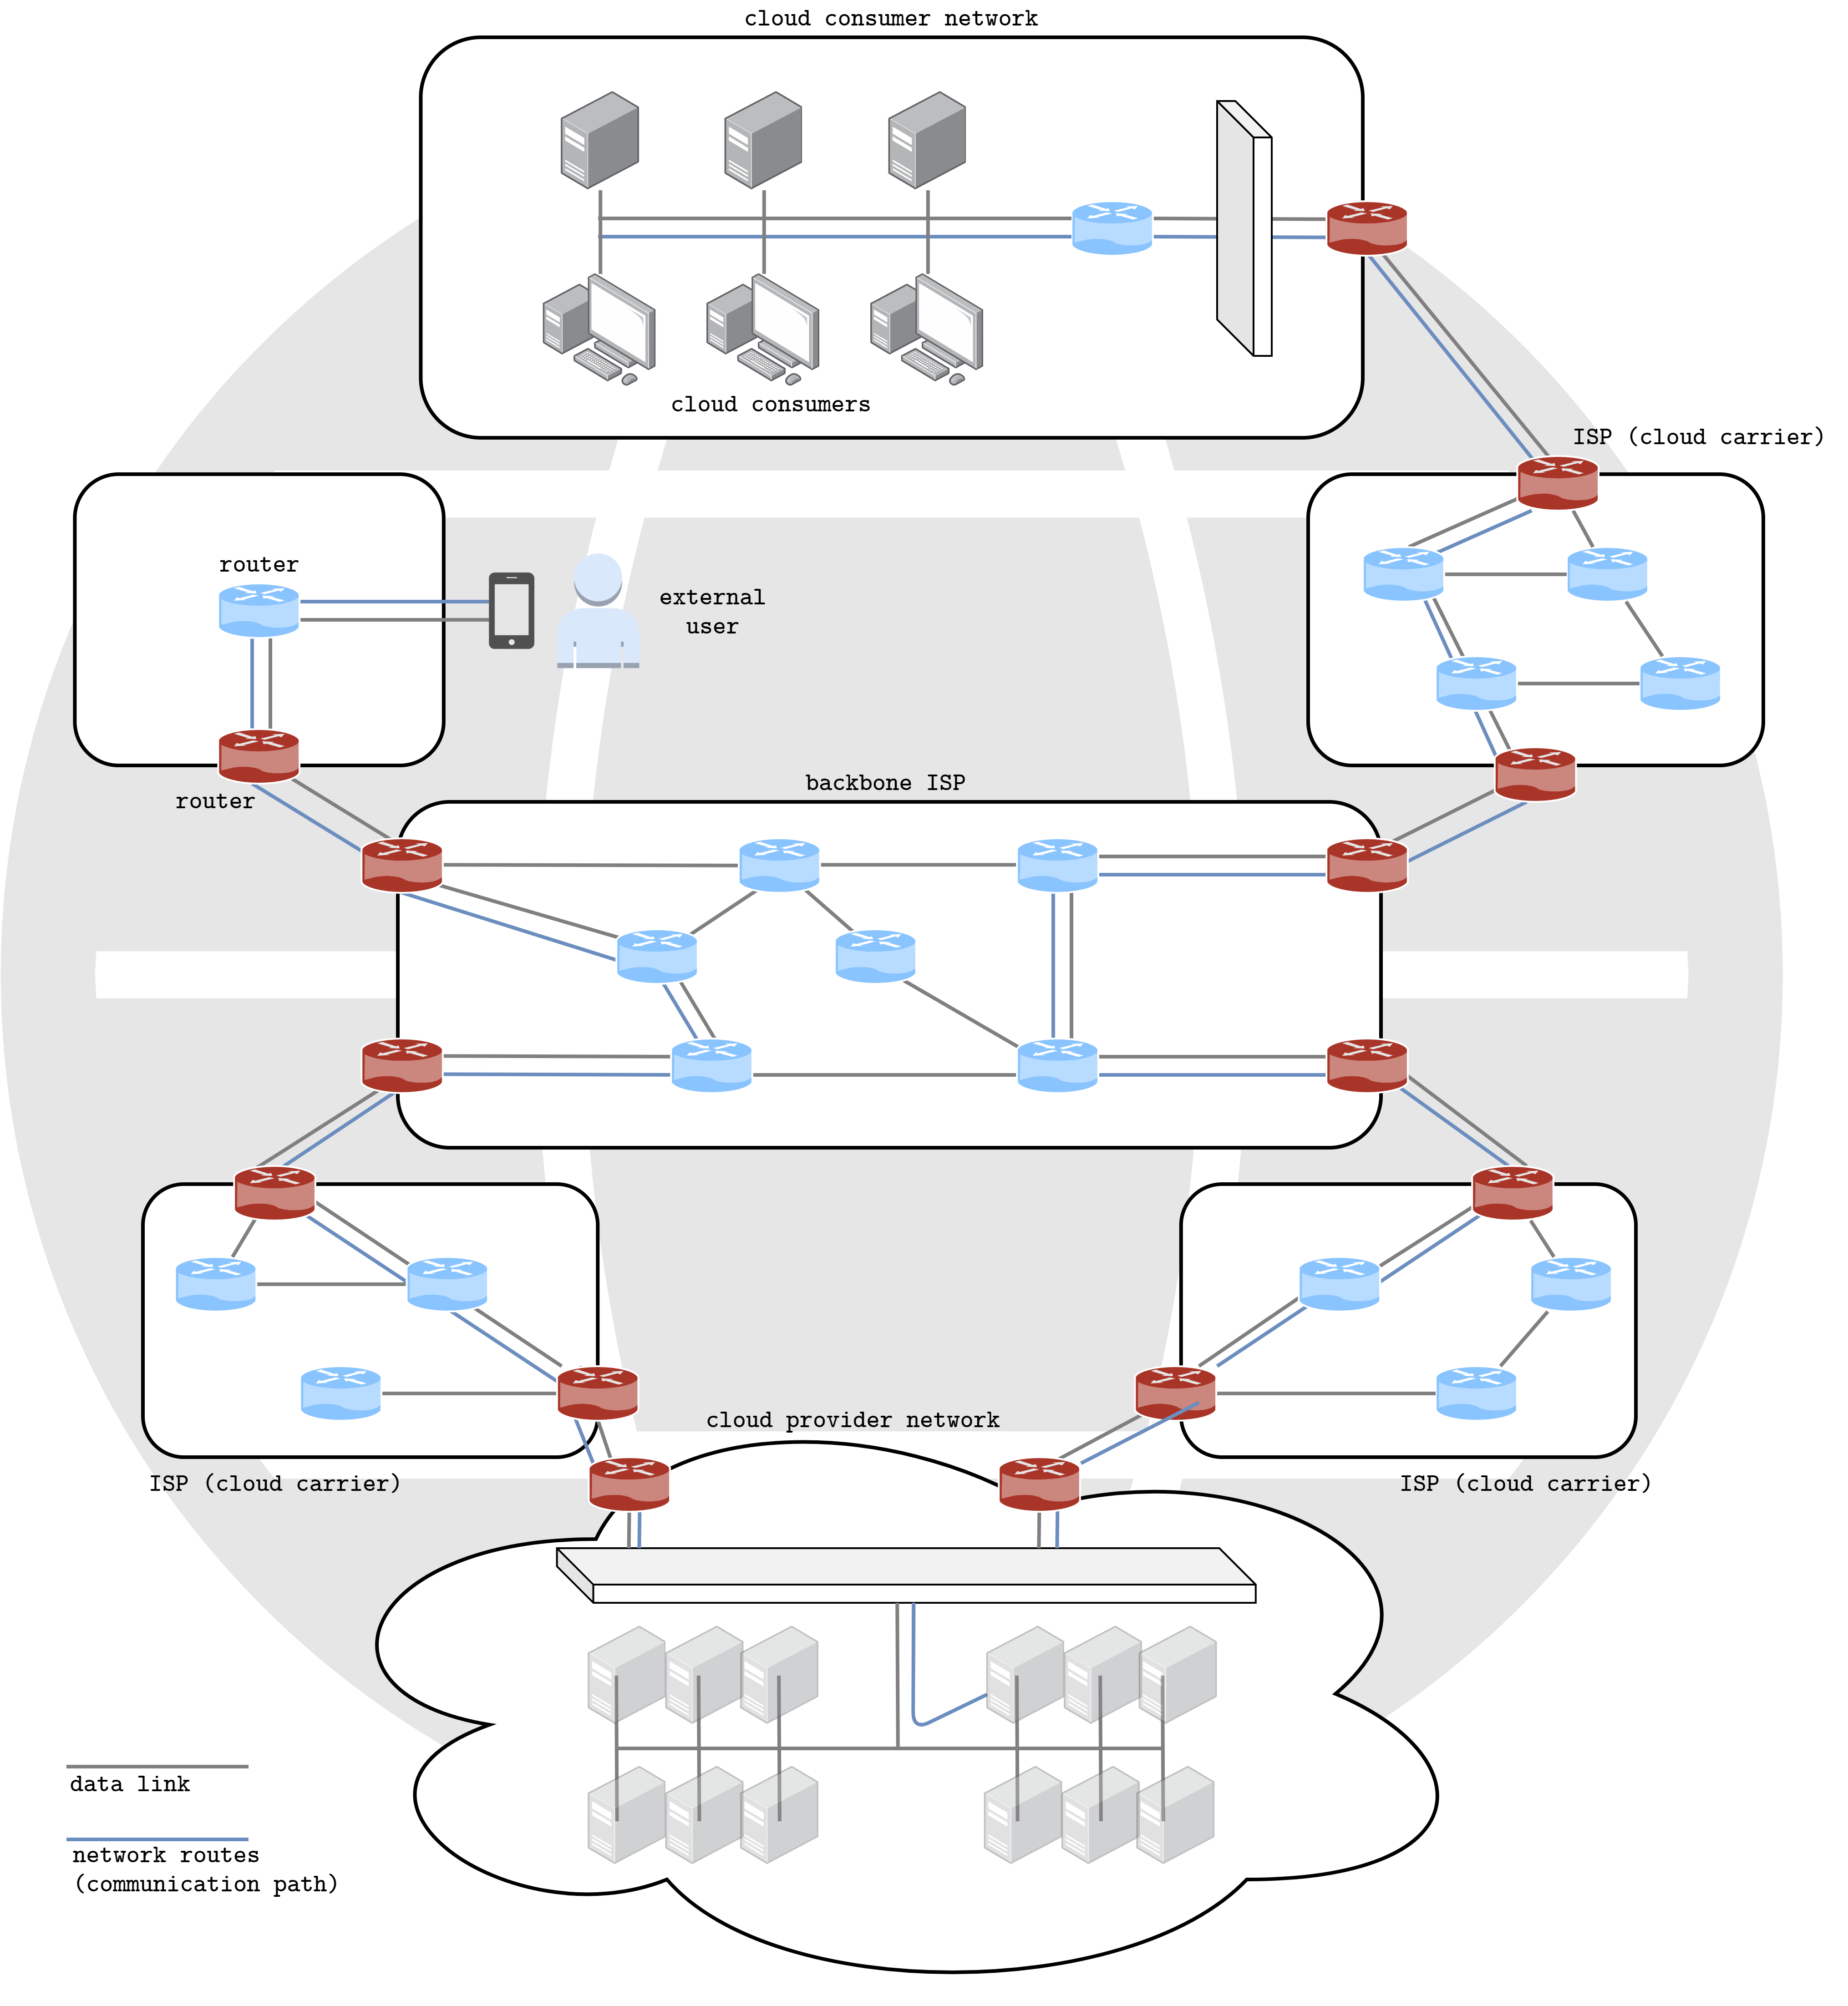
\includegraphics[width=12cm]{./Images/cap3/3.8.png}
\end{figure}


La topologia della rete è divisa in maniera gerarchica in tre Tier:
\begin{itemize}
    \item Al \textbf{Tier 1} appartengono le tecnologie di rete utilizzate per connessione con cavi sottomarini di tutto il mondo;
    \item Il \textbf{Tier 2} è rappresentato dai grandi provider regionali;
    \item Al \textbf{Tier 3} appartengono gli ISP locali (Vodafone, TIM, ecc.).
\end{itemize}

La comunicazione di rete avviene generalmente tramite protocollo TCP: è previsto il riassemblaggio di pacchetti che possono arrivare tramite diversi ISP. Il routing dei pacchetti avviene al layer 7 della pila ISO/OSI e non al layer 4 in quanto permette un load balancing migliore.

\subsection{Limitazioni e problemi}
Due punti cruciali delle comunicazioni di rete sono la latenza e la larghezza di banda: da un lato ci sono i provider che migliorano sempre di più la qualità della rete, dall'altra gli utenti che utilizzano e richiedono sempre più banda. La latenza invece rappresenta un problema perché rallenta i pacchetti nel caso di nodi congestionati. Infatti le applicazioni che si basano sulla rete spesso devono rispondere a requisiti molto stretti e che quindi vengono influenzati in maniera importante da latenza e larghezza di banda, quindi la scelta di un cloud carrier diventa importante.

\section{Data Center Technology}
I centri di calcolo si basano su alcune componenti chiave come la virtualizzazione, che permette di rendere standard e modulare la fornitura di hardware, in quanto viene fornito hardware sempre identico perché astratto. Le strutture sono basate su rack di componenti facilmente rimpiazzabili e affidabili. Alcuni di questi componenti supportano lo swap a caldo, migliorando le prestazioni, grazie all'esistenza di blade che condividono componenti critiche (gestione, console, periferiche di massa locali) che costituiscono i nodi di calcolo del data center. 

\begin{figure}[ht]
    \centering
    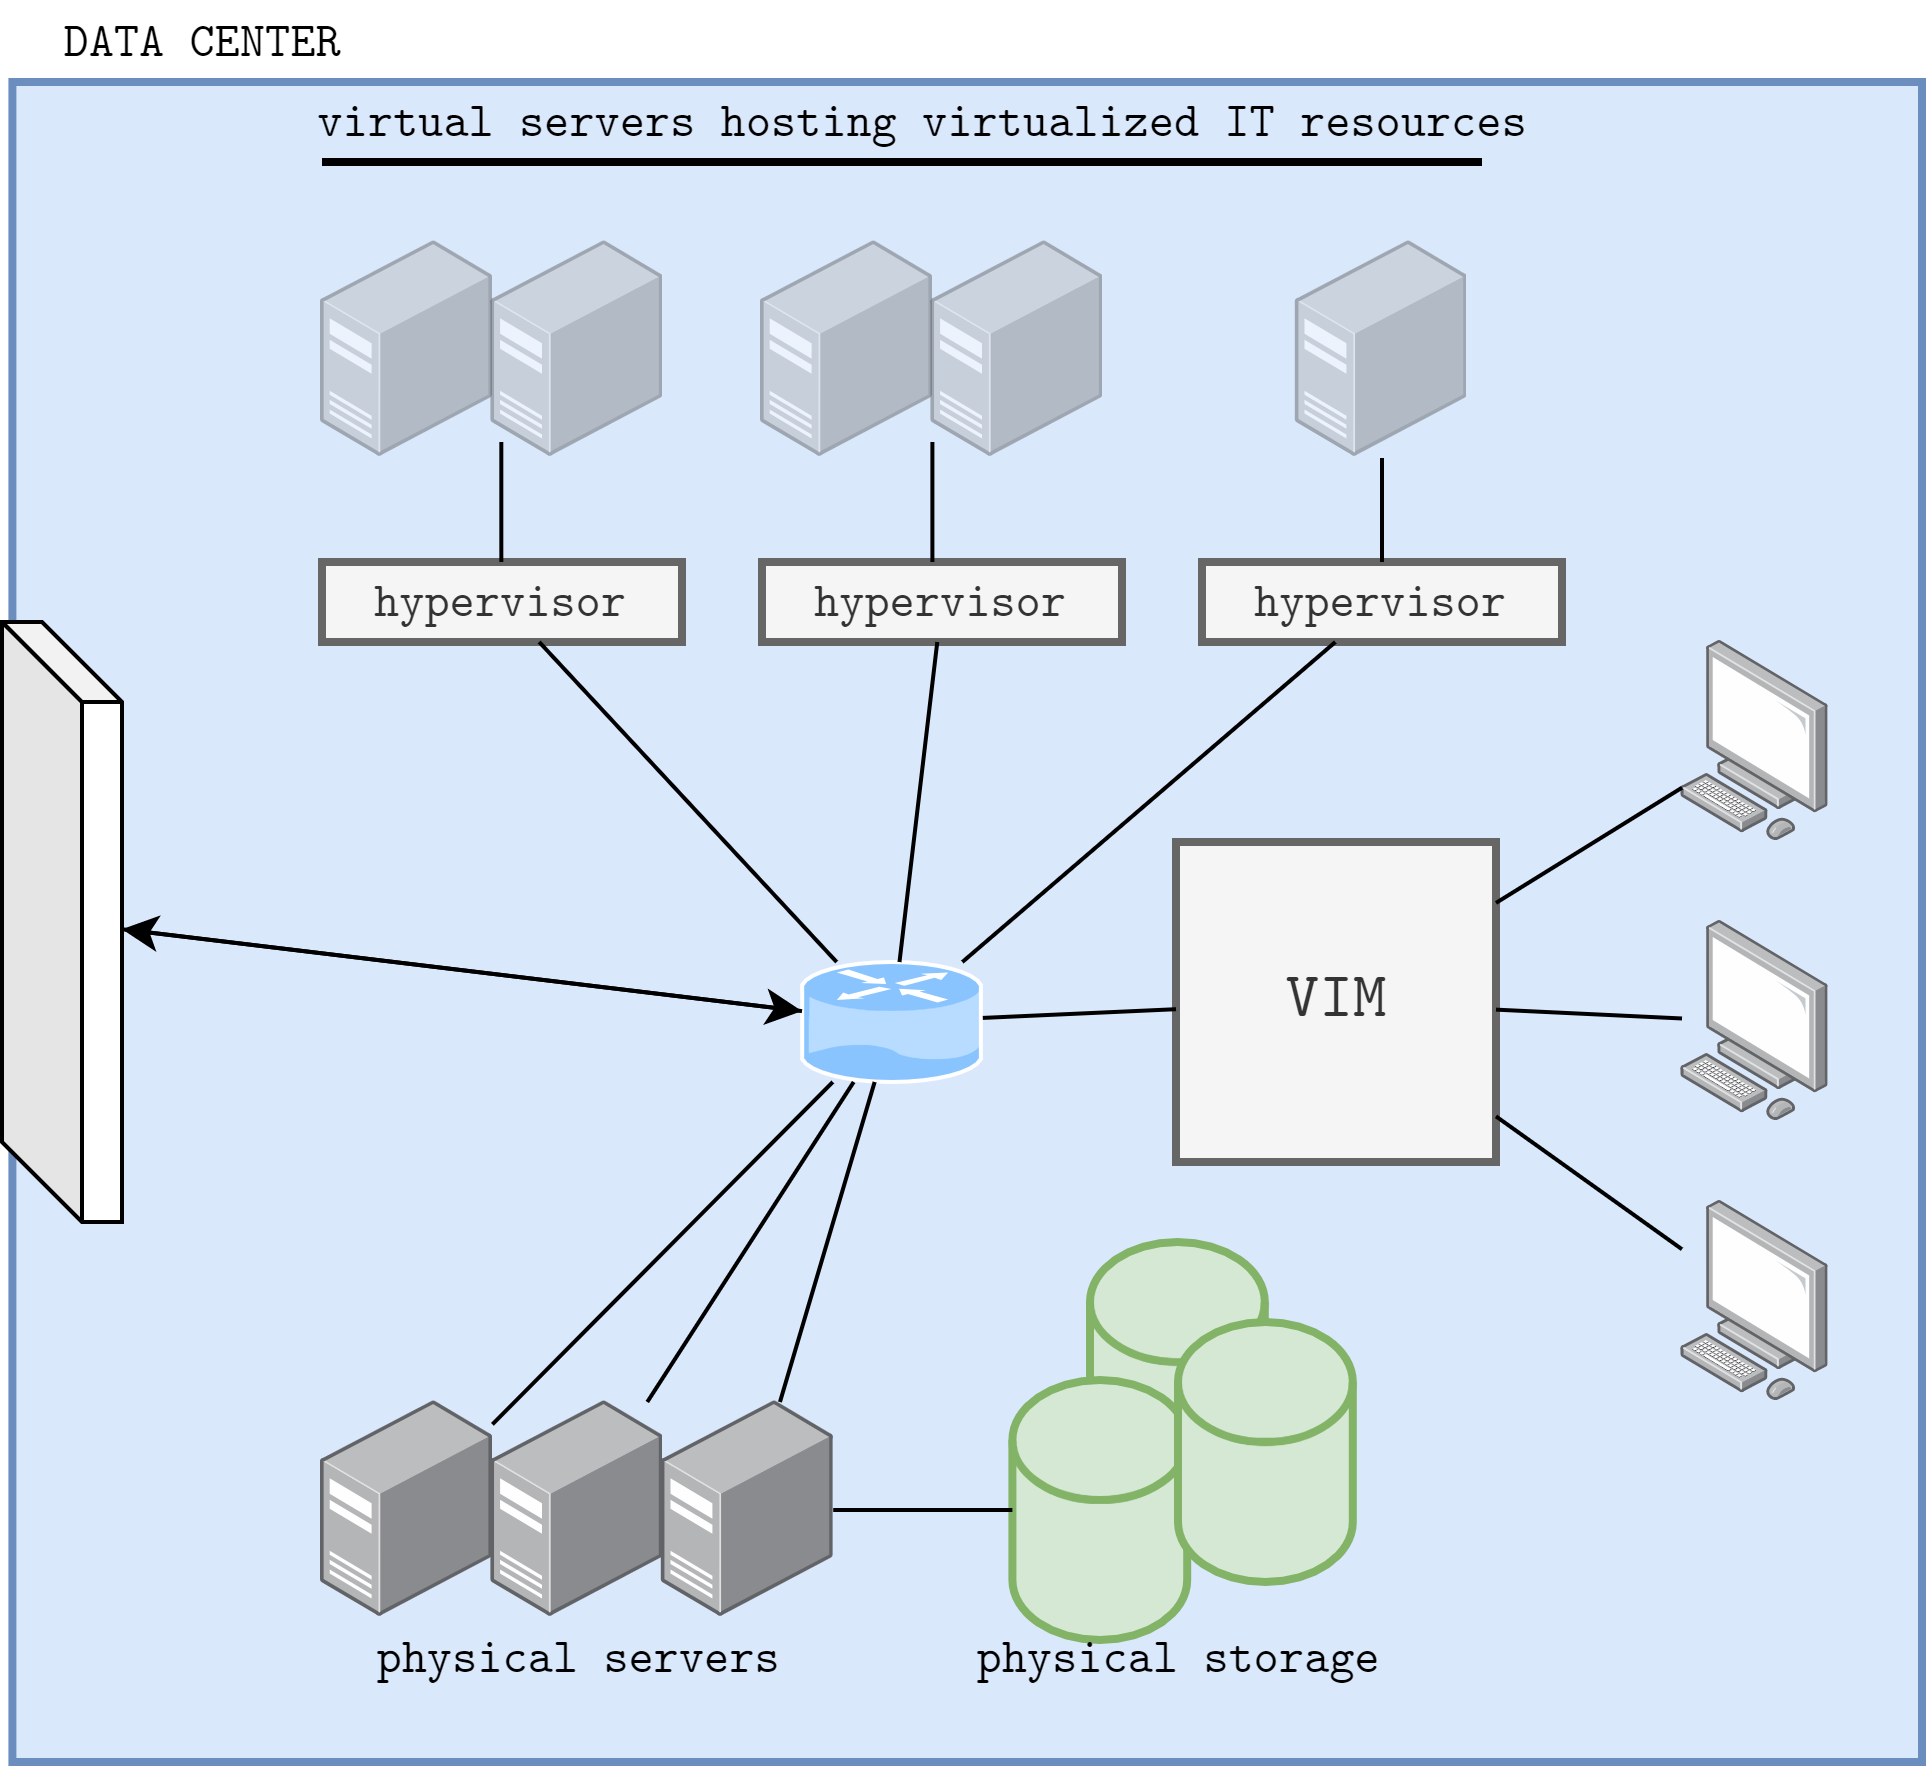
\includegraphics[width=7cm]{./Images/cap3/3.9.png}
\end{figure}

\subsection{Funzionamento}
Lo storage è organizzato in maniera ridondante, dove è possibile l'accesso sia a blocchi sia a livello di file. Le reti che vanno verso l'esterno si interconnettono direttamente con un cloud carrier, fatto con tecnologie estremamente veloci. Il load balancing, come detto anche in precedenza, avviene guardando il contenuto dei pacchetti (quindi a level 7), in questo modo si può riconoscere un certo tipo di richiesta, e se già è stata fatta in precedenza, viene inoltrata allo stesso nodo che la ha già in cache, aumentando le prestazioni.

\vspace{5mm}

I data center hanno un ciclo di vita di 5-7 anni. Per calcolare il ciclo di vita si analizzano alcuni parametri, tra cui l'ammortamento del costo, la velocità di crescita delle tecnologie, il fatto per cui i costi di gestione aumentano per macchine più vecchie: infatti un centro di calcolo è eterogeneo per definizione. La sicurezza di un data center è fondamentale perché i dati si trovano tutti in un solo posto e vanno protetti bene. I vantaggi dell'utilizzo vanno dalla condivisione dell'energia elettrica al raffreddamento, al contesto operativo, più facile da gestire a livello organizzativo.

\section{Virtualization Technology}
Virtualizzare significa portare qualcosa di fisico a livello software. È possibile virtualizzare:
\begin{itemize}
    \item server;
    \item storage: ha diversi vantaggi, ad esempio è possibile replicare dati e ottenere dischi virtuali di qualsiasi dimensione, non rimanendo vincolati dalle dimensioni dei dischi in commercio. Ad esempio è possibile virtualizzare un disco da 4.20 GB.
    \item network: incapsulando pacchetti in altri pacchetti e facendo in modo che il routing venga svolto in maniera logica;
    \item power: anche l'energia elettrica si può virtualizzare, utilizzando un UPS (Uniterrutable Power Supply).
\end{itemize}

I principali vantaggi solo l'indipendenza dall'hardware, magari attraverso server più potenti che permettono ad una stessa macchina virtuale di offrire prestazioni migliori, ma anche la possibilità di fare rollback in qualsiasi momento e con pochissimo sforzo.

Le due opzioni più diffuse sono la \textbf{OS based virtualization} e la \textbf{hardware based virtualization}. La prima è meno efficiente perché il sistema operativo consuma più risorse, e spesso finisce per rallentare la macchina a causa delle molteplici dipendenze e colli di bottiglia. Un altro problema è rappresentato dal costo delle licenze.

L'hardware based virtualization invece utilizza un \textbf{hypervisor} che non è altro che una versione molto semplificata di un sistema operativo contenente solo il minimo necessario per permettere il corretto funzionamento delle applicazioni che ci girano sopra. Permette la gestione di più virtual machine all'interno utilizzando dati ottimizzati per i server. Il tutto è organizzato da un VIrtual Infrastructure Manager (VIM). Il grafico illustra le differenze tra i due tipi di virtualizzazione.

\begin{figure}[ht]
    \centering
    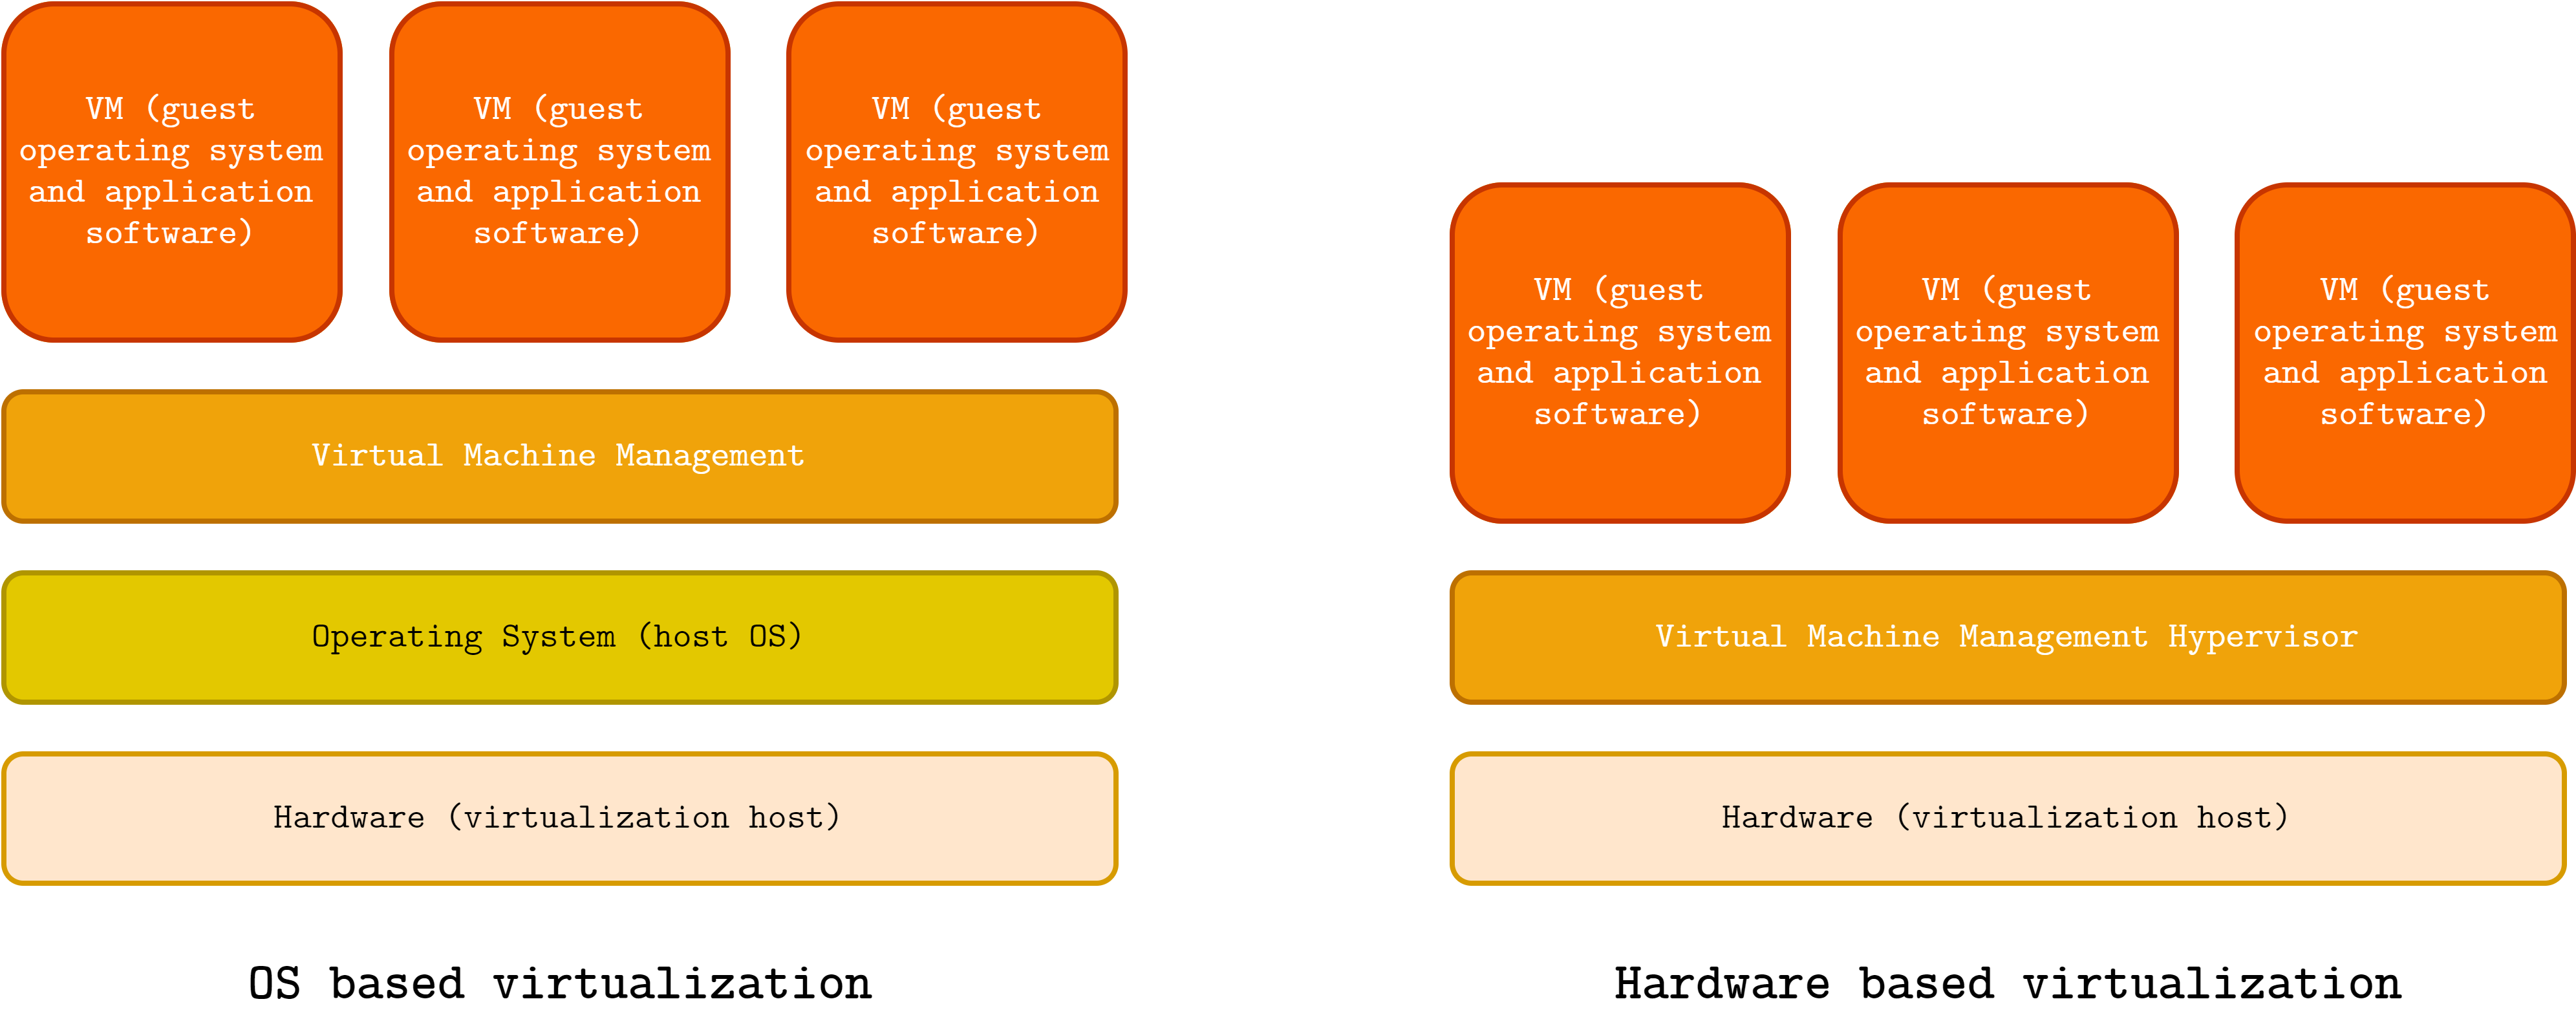
\includegraphics[width=12cm]{./Images/cap3/3.10.png}
\end{figure}

\section{Web Technology}
Le tecnologie web sono utilizzate generalmente come implementazione a livello intermedio e a livello di interfaccia per i servizi cloud based. Le componenti fondamentali del web sono il web browser client e il web server. A questi due si uniscono le strutture quali gateways, router, load balancer che ne migliorano l'affidabilità e la scalabilità. L'architettura del web si basa fondamentalmente su:
\begin{itemize}
    \item \textbf{Uniform Resource Locator (URL)}: una sintassi standard per creare identificativi che puntano a risorse web;
    \item \textbf{HyperText Transfer Protocol (HTTP)}: il protocollo principale di comunicazione utilizzato nel web;
    \item \textbf{Markup Languages (HTML, XML)}: linguaggi di etichettatura che servono a presentare graficamente le risorse accessibili.
\end{itemize}
Le applicazioni web che conosciamo sono divise in più layer, ognuno dei quali si occupa di specifici compiti. Esistono dei PaaS per tutte le applicazioni web hostate su un cloud, forniti direttamente dal cloud provider.

\section{Multitenant Technology}
Tramite la multitenant technology è possibile far accedere diversi consumer allo stesso servizio, ognuno con la propria visione dell'applicazione. Non solo, ma è possibile anche definire la gestione dell'amministrazione e della personalizzazione di un istanza di questo software condiviso, in maniera totalmente isolata tra un utente e l'altro. Principali vantaggi di questa tecnologia sono personalizzazione (UI, business process, data model), access control, data security, recovery, upgrade, data tier isolation. La differenza tra multitenancy e virtualization è essenzialmente che virtualizzazione indica stesse copie virtuali di uno stesso ambiente, mentre multitenancy indica ambienti progettati per l'accesso di diversi utenti quindi configurati in modo differente e non come semplici repliche.

\section{Service Technology}
Per Service Technology intendiamo qualsiasi tipo di tecnologia offerto come servizio. Come già spiegato precedentemente si tratta del concetto di XaaS, dove X può rappresentare qualsiasi tipo di tecnologia.
\section{Caso d'uso: DTGOV}
Analizziamo un caso d'uso, nell'ambito di DTGOV, società di pubblica amministrazione statunitense creata dal ministero della social security che serve per decentralizzare tutti i servizi di IT. Essa offre una serie di servizi per le organizzazioni del settore pubblico, sia infrastrutture IT sia software. I servizi sono personalizzati per ogni cliente, a partire dalla gestione dei contratti, fino ad arrivare alla reingegnerizzazione dei modelli IT per ridurre complessità e costi. 

L'infrastruttura comprende tre data center, uno dedicato a piattaforme low-level e altri due che offrono supporto a mainframe. I mainframe sono riservati alle attività del ministero e quindi non sono disponibili per outsourcing. Il cloud computing viene identificato come una linea guida e in particolare:
\begin{itemize}
    \item \textbf{business benefit}: cercare di standardizzare i servizi per metterli all'interno dei modelli cloud;
    \item \textbf{technical challenges}: l'infrastruttura deve adeguarsi alla fornitura di nuovi servizi;
    \item \textbf{service portfolio}: si cerca di capire cosa si può offrire e quali servizi dovrebbero diventare cloud based;
    \item \textbf{pricing and SLA}: stabilire i contratti, il prezzo e la Quality of Service.
\end{itemize}
L'azienda mette inoltre a disposizione dei servizi di migrazione che convincano utenti e aziende a migrare verso il cloud. Viene stabilita una roadmap: dopo alcuni survey viene scelta la target delivery platform per iniziare l'attività del lavoro di migrazione, per poi identificare un'azienda per guidare questo processo. In breve quest'azienda sta diventando pian piano fornitore di servizi cloud per le pubbliche amministrazioni.

\section{Learning Check}
\begin{enumerate}
    \item Descrivi la relazione tra le reti a banda larga e gli ISP e il Cloud computing.
    \item Spiega come funziona il \textit{connectionless packet switching}, l'interconnettività router-based e i protocolli a livello di trasporto e a livello di applicazione.
    \item Spiega perché i problemi che riguardano larghezza di banda e latenza sono comuni nell'architettura di Internet.
    \item Descrivi la data center technology e la sua rilevanza oggi nel cloud computing.
    \item Sempre per quanto riguarda i data center, spiega la standardizzazione, la modularità, l'automazione e il controllo remoto.
    \item Spiega l'importanza della \textit{high availability} e della security nei data center e le componenti hardware e dei servizi primari di un data center.
    \item Spiega l'importanza contemporanea della virtualization technology nel cloud computing, indicando perchè sono importanti l'indipendenza dall'hardware, la \textit{server consolidation} e la replicazione delle risorse.
    \item Spiega la differenza tra la virtualizzazione OS e hardware-based.
    \item Descrivi la rilevanza delle tecnologie web e le applicazioni web-based nel cloud computing.
    \item Descrivi la \textit{multitenancy} e l'importanza della multitenant technology nel cloud computing.
    \item Descrivi le principali service technologies e la loro importanza nel cloud computing, includendo i servizi web SOAP-based, i servizi REST, i service agents e i service middleware.
    \item Descrivi quali sono le tecnologie e gli standard più diffusi per lo sviluppo di servizi web.
    \item Descrivi i servizi REST e spiega come sono in relazione con un contratto uniforme fornito dai metodi di HTTP.
\end{enumerate}
